		\subsection{Chart}

		\begin{frame}
		
		
		\begin{CaixaModelo01}{Graficos}
			
Exemplo Sofisticado:\\
https://www.codeproject.com/Articles/32836/A-simple-C-library-for-graph-plotting

	\begin{columns}
		\begin{column}{0.33\textwidth}
			\begin{figure}
				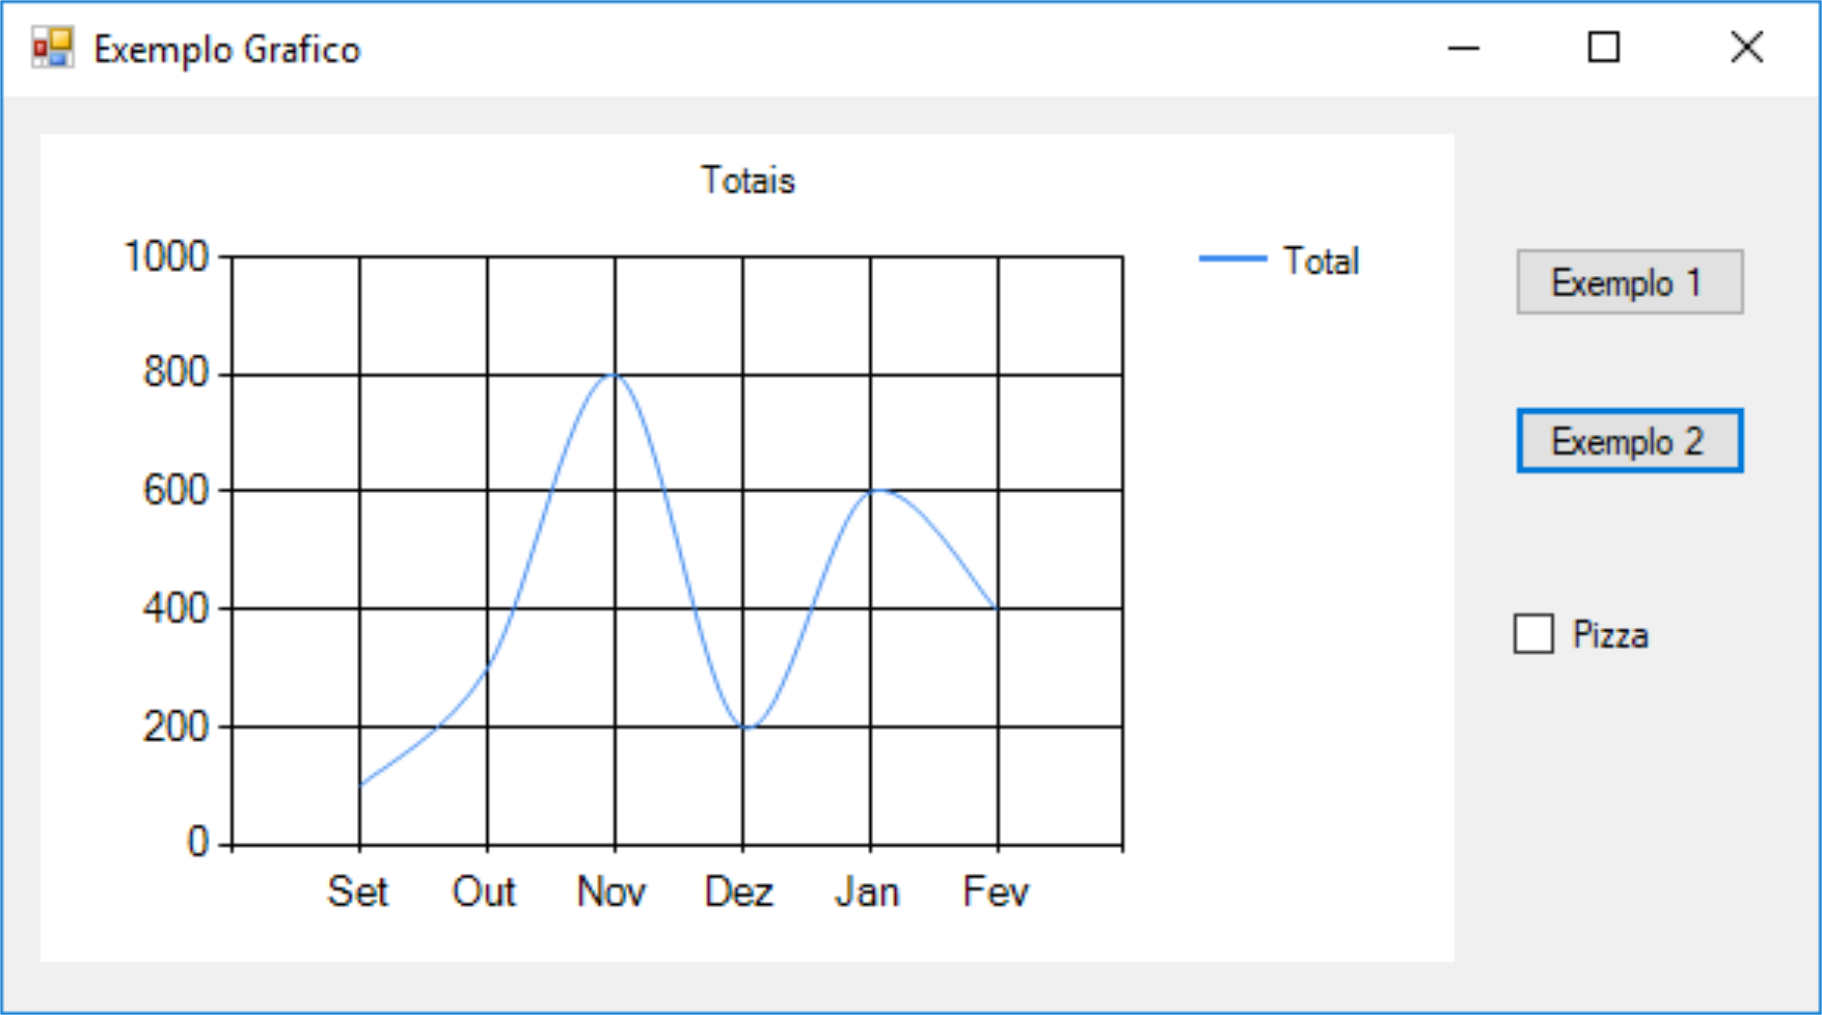
\includegraphics[scale=.2]{./Figuras/Grafico01}
				\caption{Grafico Estilo Linhas}
				\label{fig:Grafico01}
			\end{figure}
		\end{column}
		\begin{column}{0.33\textwidth}
			\begin{figure}
				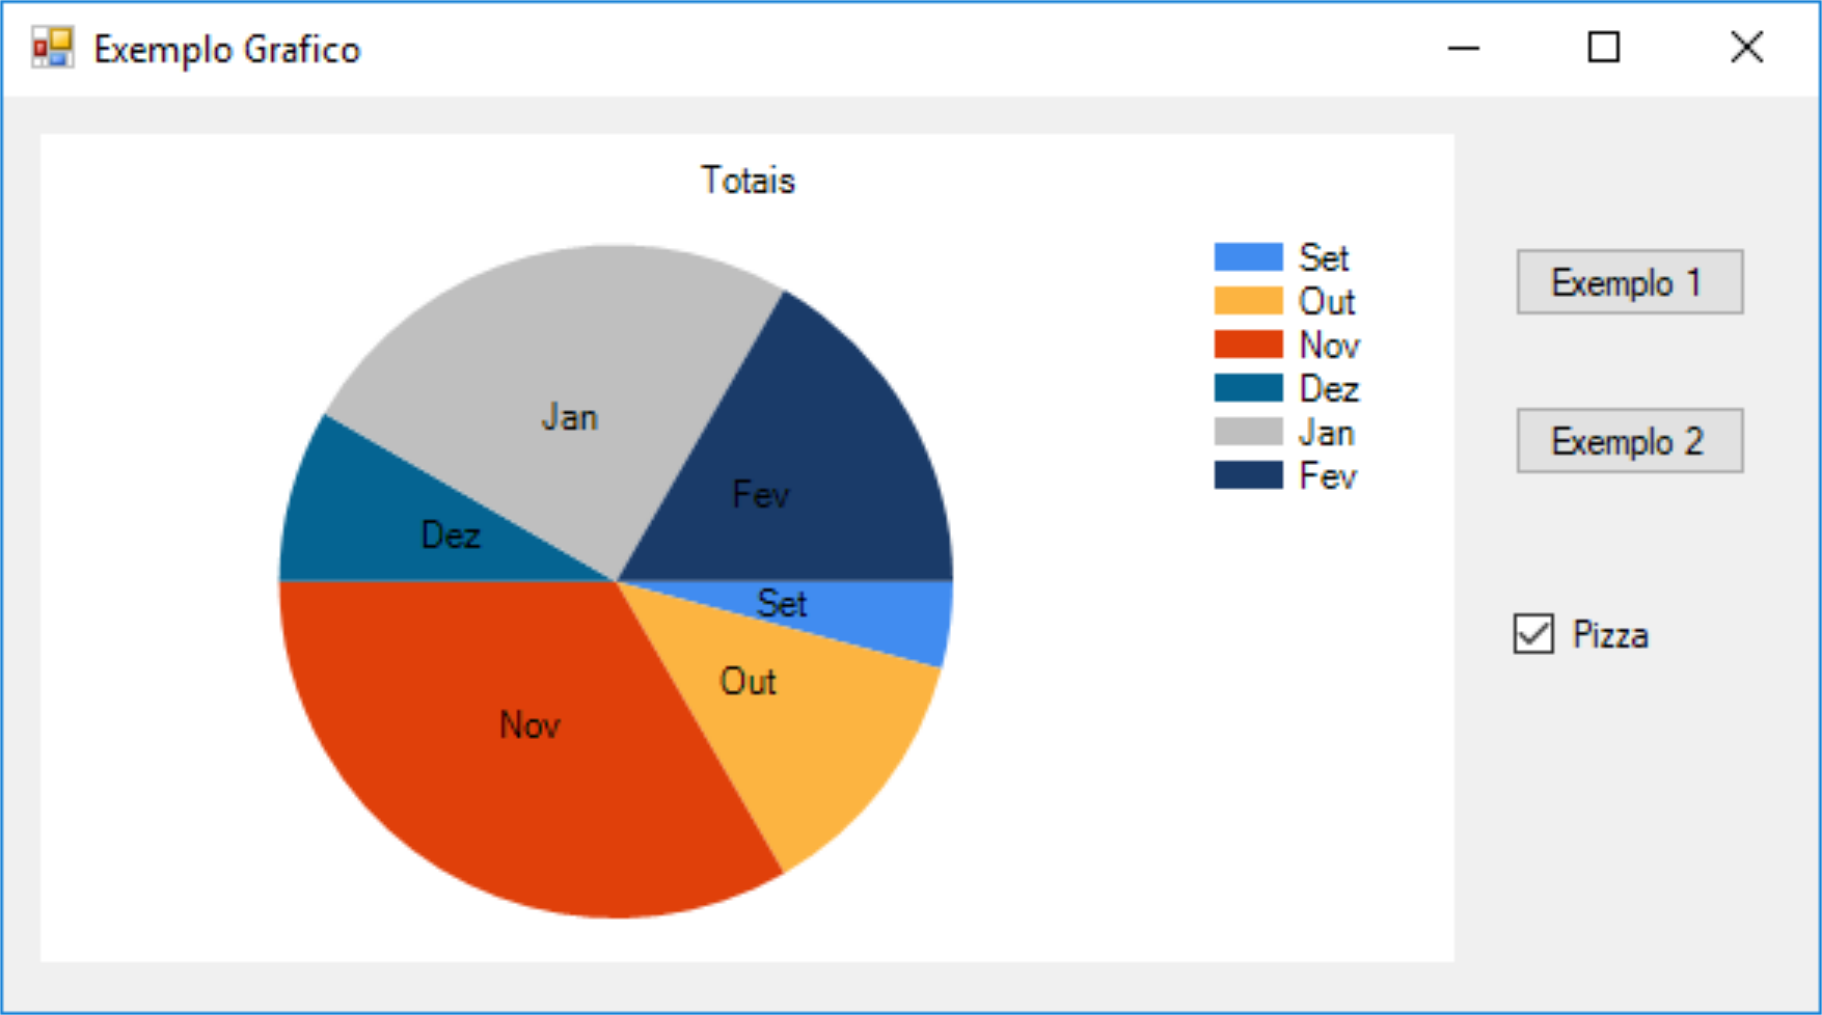
\includegraphics[scale=.2]{./Figuras/Grafico02}
				\caption{Grafico Estilo Pizza}
				\label{fig:Grafico02}
			\end{figure}
		\end{column}
		\begin{column}{0.33\textwidth}
			\begin{figure}
				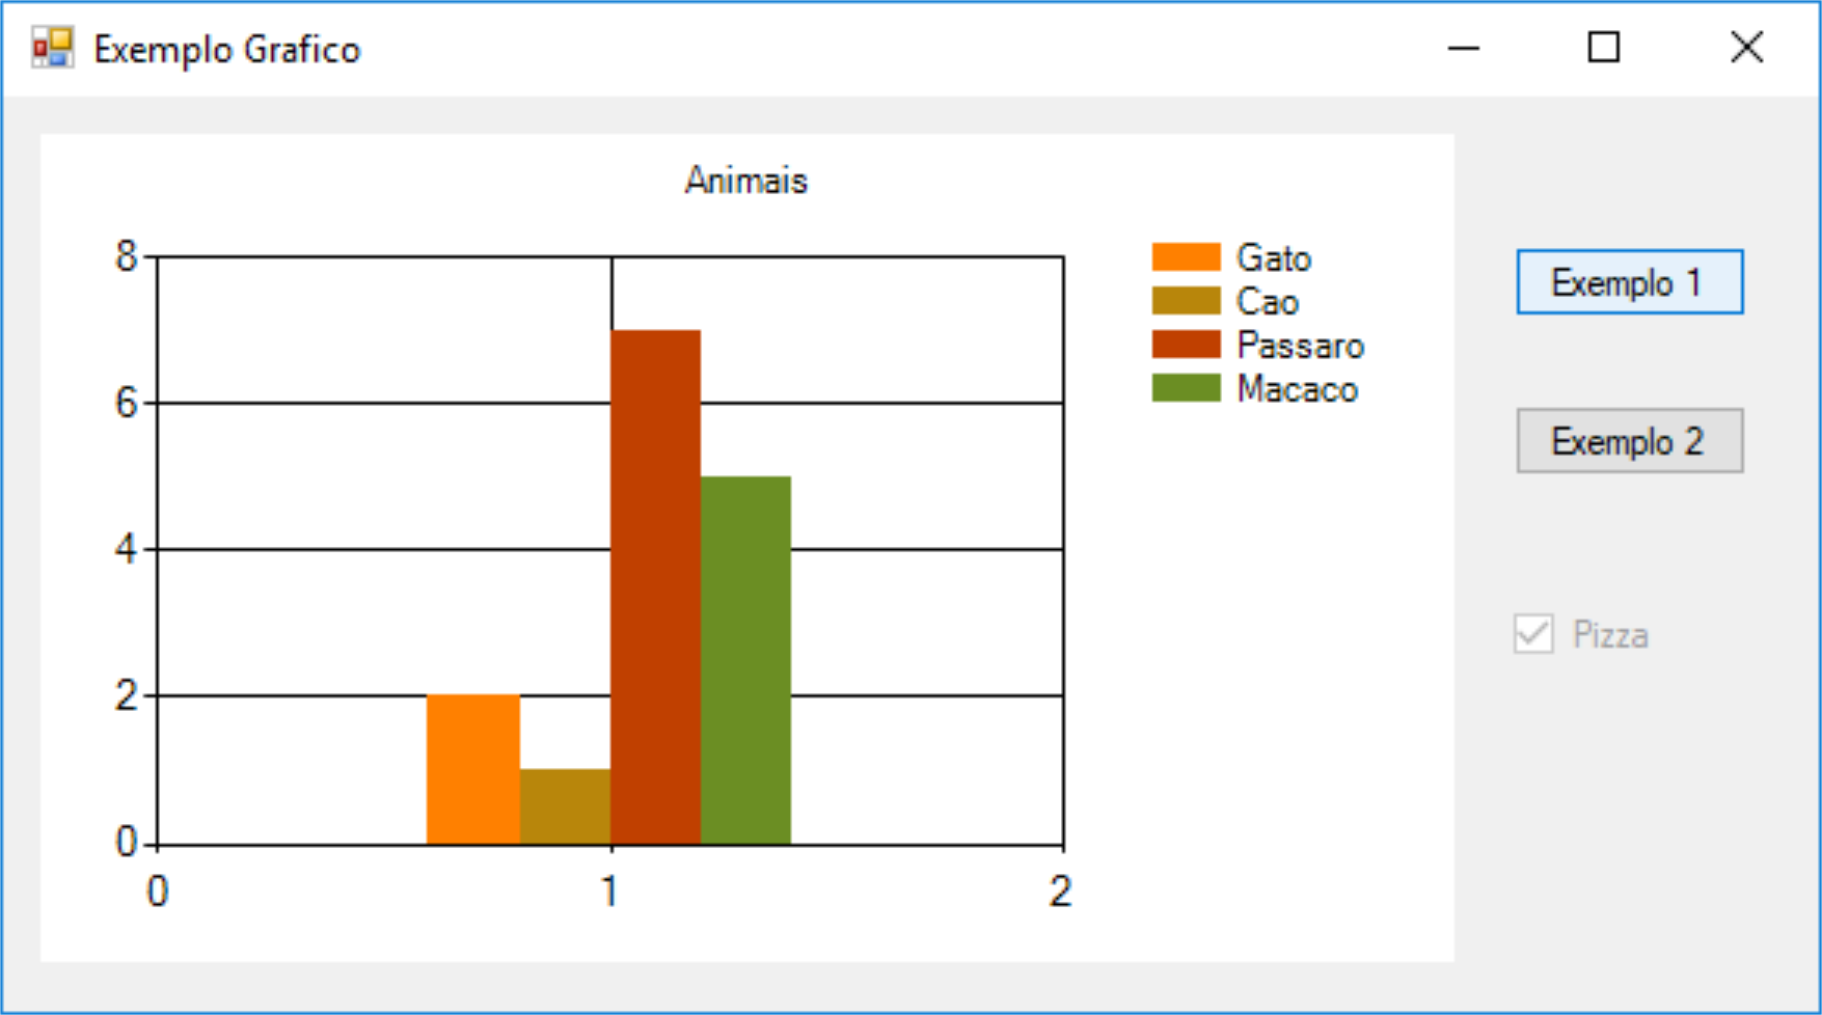
\includegraphics[scale=.2]{./Figuras/Grafico03}
				\caption{Gráfico Estilo Barras}
				\label{fig:Grafico03}
			\end{figure}
	\end{column}
	\end{columns}	
	\end{CaixaModelo01}
			
	   \end{frame}
		